\documentclass[tikz,border=0pt]{standalone}
\usepackage{xcolor}
\usetikzlibrary{calc}
% Palette: Sam_Comm_final.png by eye, and the drones and raiders.
\definecolor{ink}{HTML}{3B2340}
\definecolor{sky}{HTML}{EFC46A}
\definecolor{skyhi}{HTML}{F5DA92}
\definecolor{skylow}{HTML}{E9B060}
\definecolor{cloud}{HTML}{F2D58A}
\definecolor{paper}{HTML}{FBEFD0}
\definecolor{cream}{HTML}{FFF6E0}
\definecolor{white}{HTML}{FFFFFF}
\definecolor{wallA}{HTML}{E88A73}
\definecolor{wallB}{HTML}{EE9F7E}
\definecolor{wallC}{HTML}{E47A7E}
\definecolor{wallD}{HTML}{F0B07E}
\definecolor{wallE}{HTML}{D9765F}
\definecolor{wallF}{HTML}{E99A8A}
\definecolor{greenA}{HTML}{8DBB7E}
\definecolor{greenB}{HTML}{6FA77A}
\definecolor{greenC}{HTML}{A9C97F}
\definecolor{greenD}{HTML}{5E9C6A}
\definecolor{greenE}{HTML}{4A8060}
\definecolor{sage}{HTML}{9DB98A}
\definecolor{sagedark}{HTML}{6F8F66}
\definecolor{sagelight}{HTML}{C2D6A6}
\definecolor{window}{HTML}{F6E7A0}
\definecolor{windark}{HTML}{8C5A64}
\definecolor{metal}{HTML}{8D9A93}
\definecolor{metaldark}{HTML}{5E6B66}
\definecolor{metallight}{HTML}{B9C4BC}
\definecolor{wood}{HTML}{B9835A}
\definecolor{wooddark}{HTML}{8C5A3C}
\definecolor{woodlight}{HTML}{D9A66F}
\definecolor{stone}{HTML}{E7C9A0}
\definecolor{stonedark}{HTML}{C9A47E}
\definecolor{concrete}{HTML}{D8C3A4}
\definecolor{concretedark}{HTML}{B8A084}
\definecolor{asphalt}{HTML}{8E7A86}
\definecolor{asphaltdark}{HTML}{6E5C68}
\definecolor{roadline}{HTML}{F6E7A0}
\definecolor{kerb}{HTML}{D8B48C}
\definecolor{red}{HTML}{E0483E}
\definecolor{redlight}{HTML}{F27A6A}
\definecolor{gold}{HTML}{FFB000}
\definecolor{goldlight}{HTML}{FFD54F}
\definecolor{teal}{HTML}{4FA3A0}
\definecolor{tealdark}{HTML}{3C8582}
\definecolor{magenta}{HTML}{FF2E88}
\definecolor{cyan}{HTML}{13CFE3}
\definecolor{violet}{HTML}{8A5BD6}
\definecolor{orange}{HTML}{F2803A}
\definecolor{pink}{HTML}{F48FB1}
\definecolor{glow}{HTML}{4FE6E0}
\definecolor{glowhi}{HTML}{C8FFF9}
\definecolor{hot}{HTML}{FF6A1A}
\definecolor{hothi}{HTML}{FFD07A}
\definecolor{armour}{HTML}{7E7A86}
\definecolor{armourdark}{HTML}{5A5466}
\definecolor{armourlight}{HTML}{A8A2B0}
\definecolor{wasp}{HTML}{E0A82E}
\definecolor{waspdark}{HTML}{B07E1A}
\definecolor{moth}{HTML}{F2E6C8}
\definecolor{mothdark}{HTML}{D2C09A}
\definecolor{hornet}{HTML}{3C8582}
\definecolor{hornetdark}{HTML}{2C6260}
\definecolor{warden}{HTML}{E47A7E}
\definecolor{wardendark}{HTML}{B85A62}
\definecolor{tick}{HTML}{8DBB7E}
\definecolor{tickdark}{HTML}{5E8A5A}
\definecolor{strider}{HTML}{D9765F}
\definecolor{striderdark}{HTML}{A8543F}
\definecolor{jacket}{HTML}{6FA77A}
\definecolor{jacketb}{HTML}{4FA3A0}
\definecolor{jacketc}{HTML}{E88A73}
\definecolor{jacketd}{HTML}{F0B07E}
\definecolor{skin}{HTML}{F2C49A}
\definecolor{skinb}{HTML}{C98C6A}
\definecolor{skinc}{HTML}{8C5A3C}
\definecolor{hair}{HTML}{3B2340}
\definecolor{goo}{HTML}{B6E35A}
\definecolor{goodark}{HTML}{7FB23A}
\newcommand{\Ink}{1.8pt}
\tikzset{inked/.style={draw=ink, line width=\Ink, line join=round, line cap=round}}
\begin{document}
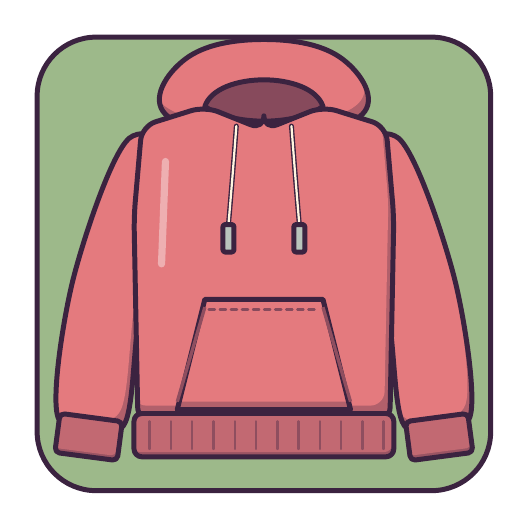
\begin{tikzpicture}
\clip (0,0) rectangle (6,6);
\fill[sage] [rounded corners=0.75cm] (0.12,0.12) rectangle (5.88,5.88);
\begin{scope}\clip [rounded corners=0.75cm] (0.12,0.12) rectangle (5.88,5.88);
\begin{scope}\clip plot[smooth cycle, tension=0.7] coordinates {(1.75,4.9) (2,5.6) (3,5.85) (4,5.6) (4.25,4.9) (3,4.6)};
\fill[wallC!70!ink] plot[smooth cycle, tension=0.7] coordinates {(1.75,4.9) (2,5.6) (3,5.85) (4,5.6) (4.25,4.9) (3,4.6)};
\fill[wallC, shift={(-0.049,0.14)}] plot[smooth cycle, tension=0.7] coordinates {(1.75,4.9) (2,5.6) (3,5.85) (4,5.6) (4.25,4.9) (3,4.6)};
\end{scope}
\draw[inked] plot[smooth cycle, tension=0.7] coordinates {(1.75,4.9) (2,5.6) (3,5.85) (4,5.6) (4.25,4.9) (3,4.6)};
\filldraw[inked, fill=wallC!45!ink] (2.25,5.0) .. controls (2.4,5.45) and (3.6,5.45) .. (3.75,5.0) .. controls (3.4,4.75) and (2.6,4.75) .. (2.25,5.0) -- cycle;
\begin{scope}\clip plot[smooth cycle, tension=0.5] coordinates {(4.71,4.596) (5.418,2.824) (5.616,1.055) (4.784,0.945) (4.532,2.576) (3.79,4.204)};
\fill[wallC!70!ink] plot[smooth cycle, tension=0.5] coordinates {(4.71,4.596) (5.418,2.824) (5.616,1.055) (4.784,0.945) (4.532,2.576) (3.79,4.204)};
\fill[wallC, shift={(-0.056,0.16)}] plot[smooth cycle, tension=0.5] coordinates {(4.71,4.596) (5.418,2.824) (5.616,1.055) (4.784,0.945) (4.532,2.576) (3.79,4.204)};
\end{scope}
\draw[inked] plot[smooth cycle, tension=0.5] coordinates {(4.71,4.596) (5.418,2.824) (5.616,1.055) (4.784,0.945) (4.532,2.576) (3.79,4.204)};
\begin{scope}\clip[rounded corners=0.06cm] (5.589,1.102) -- (5.655,0.606) -- (4.863,0.502) -- (4.798,0.997) -- cycle;
\fill[wallC!80!ink!70!ink,rounded corners=0.06cm] (5.589,1.102) -- (5.655,0.606) -- (4.863,0.502) -- (4.798,0.997) -- cycle;
\fill[wallC!80!ink,rounded corners=0.06cm, shift={(-0.021,0.06)}] (5.589,1.102) -- (5.655,0.606) -- (4.863,0.502) -- (4.798,0.997) -- cycle;
\end{scope}
\draw[inked,rounded corners=0.06cm] (5.589,1.102) -- (5.655,0.606) -- (4.863,0.502) -- (4.798,0.997) -- cycle;
\begin{scope}\clip plot[smooth cycle, tension=0.5] coordinates {(2.21,4.204) (1.468,2.576) (1.216,0.945) (0.384,1.055) (0.582,2.824) (1.29,4.596)};
\fill[wallC!70!ink] plot[smooth cycle, tension=0.5] coordinates {(2.21,4.204) (1.468,2.576) (1.216,0.945) (0.384,1.055) (0.582,2.824) (1.29,4.596)};
\fill[wallC, shift={(-0.056,0.16)}] plot[smooth cycle, tension=0.5] coordinates {(2.21,4.204) (1.468,2.576) (1.216,0.945) (0.384,1.055) (0.582,2.824) (1.29,4.596)};
\end{scope}
\draw[inked] plot[smooth cycle, tension=0.5] coordinates {(2.21,4.204) (1.468,2.576) (1.216,0.945) (0.384,1.055) (0.582,2.824) (1.29,4.596)};
\begin{scope}\clip[rounded corners=0.06cm] (1.202,0.997) -- (1.137,0.502) -- (0.345,0.606) -- (0.411,1.102) -- cycle;
\fill[wallC!80!ink!70!ink,rounded corners=0.06cm] (1.202,0.997) -- (1.137,0.502) -- (0.345,0.606) -- (0.411,1.102) -- cycle;
\fill[wallC!80!ink,rounded corners=0.06cm, shift={(-0.021,0.06)}] (1.202,0.997) -- (1.137,0.502) -- (0.345,0.606) -- (0.411,1.102) -- cycle;
\end{scope}
\draw[inked,rounded corners=0.06cm] (1.202,0.997) -- (1.137,0.502) -- (0.345,0.606) -- (0.411,1.102) -- cycle;
\begin{scope}\clip [rounded corners=0.18cm] (3,4.7) -- (3.75,5) -- (4.55,4.75) -- (4.65,3.6) -- (4.6,1) -- (3,1) -- (3,1) -- (1.4,1) -- (1.35,3.6) -- (1.45,4.75) -- (2.25,5) -- (3,4.7) -- cycle;
\fill[wallC!70!ink] [rounded corners=0.18cm] (3,4.7) -- (3.75,5) -- (4.55,4.75) -- (4.65,3.6) -- (4.6,1) -- (3,1) -- (3,1) -- (1.4,1) -- (1.35,3.6) -- (1.45,4.75) -- (2.25,5) -- (3,4.7) -- cycle;
\fill[wallC, shift={(-0.07,0.2)}] [rounded corners=0.18cm] (3,4.7) -- (3.75,5) -- (4.55,4.75) -- (4.65,3.6) -- (4.6,1) -- (3,1) -- (3,1) -- (1.4,1) -- (1.35,3.6) -- (1.45,4.75) -- (2.25,5) -- (3,4.7) -- cycle;
\end{scope}
\draw[inked] [rounded corners=0.18cm] (3,4.7) -- (3.75,5) -- (4.55,4.75) -- (4.65,3.6) -- (4.6,1) -- (3,1) -- (3,1) -- (1.4,1) -- (1.35,3.6) -- (1.45,4.75) -- (2.25,5) -- (3,4.7) -- cycle;
\begin{scope}\clip[rounded corners=0.1cm] (1.35,0.55) rectangle (4.65,1.1);
\fill[wallC!80!ink!70!ink,rounded corners=0.1cm] (1.35,0.55) rectangle (4.65,1.1);
\fill[wallC!80!ink,rounded corners=0.1cm, shift={(-0.021,0.06)}] (1.35,0.55) rectangle (4.65,1.1);
\end{scope}
\draw[inked,rounded corners=0.1cm] (1.35,0.55) rectangle (4.65,1.1);
\draw[wallC!50!ink, line width=0.9pt, line cap=round] (1.55,0.65) -- (1.55,1);
\draw[wallC!50!ink, line width=0.9pt, line cap=round] (1.82,0.65) -- (1.82,1);
\draw[wallC!50!ink, line width=0.9pt, line cap=round] (2.09,0.65) -- (2.09,1);
\draw[wallC!50!ink, line width=0.9pt, line cap=round] (2.36,0.65) -- (2.36,1);
\draw[wallC!50!ink, line width=0.9pt, line cap=round] (2.63,0.65) -- (2.63,1);
\draw[wallC!50!ink, line width=0.9pt, line cap=round] (2.9,0.65) -- (2.9,1);
\draw[wallC!50!ink, line width=0.9pt, line cap=round] (3.17,0.65) -- (3.17,1);
\draw[wallC!50!ink, line width=0.9pt, line cap=round] (3.44,0.65) -- (3.44,1);
\draw[wallC!50!ink, line width=0.9pt, line cap=round] (3.71,0.65) -- (3.71,1);
\draw[wallC!50!ink, line width=0.9pt, line cap=round] (3.98,0.65) -- (3.98,1);
\draw[wallC!50!ink, line width=0.9pt, line cap=round] (4.25,0.65) -- (4.25,1);
\draw[wallC!50!ink, line width=0.9pt, line cap=round] (4.52,0.65) -- (4.52,1);
\begin{scope}\clip (1.9,1.15) -- (4.1,1.15) -- (3.75,2.55) -- (2.25,2.55) -- cycle;
\fill[wallC!70!ink] (1.9,1.15) -- (4.1,1.15) -- (3.75,2.55) -- (2.25,2.55) -- cycle;
\fill[wallC, shift={(-0.035,0.1)}] (1.9,1.15) -- (4.1,1.15) -- (3.75,2.55) -- (2.25,2.55) -- cycle;
\end{scope}
\draw[inked] (1.9,1.15) -- (4.1,1.15) -- (3.75,2.55) -- (2.25,2.55) -- cycle;
\draw[wallC!50!ink, line width=1.2pt] (1.9,1.25) -- (2.25,2.45) (4.1,1.25) -- (3.75,2.45);
\draw[wallC!45!ink, line width=0.9pt, line cap=round, dash pattern=on 2.2pt off 1.8pt] (2.3,2.42) -- (3.7,2.42);
\draw[ink, line width=1.8pt, line cap=round, line join=round] plot[smooth, tension=0.6] coordinates {(2.65,4.75) (2.6,4.1) (2.55,3.5)};
\draw[cream, line width=0.8pt, line cap=round, line join=round] plot[smooth, tension=0.6] coordinates {(2.65,4.75) (2.6,4.1) (2.55,3.5)};
\begin{scope}\clip[rounded corners=0.03cm] (2.48,3.15) rectangle (2.62,3.5);
\fill[metallight!70!ink,rounded corners=0.03cm] (2.48,3.15) rectangle (2.62,3.5);
\fill[metallight,rounded corners=0.03cm, shift={(-0.007,0.02)}] (2.48,3.15) rectangle (2.62,3.5);
\end{scope}
\draw[inked,rounded corners=0.03cm] (2.48,3.15) rectangle (2.62,3.5);
\draw[ink, line width=1.8pt, line cap=round, line join=round] plot[smooth, tension=0.6] coordinates {(3.35,4.75) (3.4,4.1) (3.45,3.5)};
\draw[cream, line width=0.8pt, line cap=round, line join=round] plot[smooth, tension=0.6] coordinates {(3.35,4.75) (3.4,4.1) (3.45,3.5)};
\begin{scope}\clip[rounded corners=0.03cm] (3.38,3.15) rectangle (3.52,3.5);
\fill[metallight!70!ink,rounded corners=0.03cm] (3.38,3.15) rectangle (3.52,3.5);
\fill[metallight,rounded corners=0.03cm, shift={(-0.007,0.02)}] (3.38,3.15) rectangle (3.52,3.5);
\end{scope}
\draw[inked,rounded corners=0.03cm] (3.38,3.15) rectangle (3.52,3.5);
\draw[white, line width=2.6pt, line cap=round, line join=round, opacity=0.4] plot[smooth, tension=0.6] coordinates {(1.75,4.3) (1.7,3)};
\end{scope}
\draw[inked] [rounded corners=0.75cm] (0.12,0.12) rectangle (5.88,5.88);
\end{tikzpicture}
\end{document}
